\documentclass[
  11pt,
  letterpaper,
   addpoints,
   answers
  ]{exam}

\usepackage{../exercise-preamble}

\begin{document}

\noindent
\begin{minipage}{0.47\textwidth}

\includegraphics[width=\textwidth]{../fcfm_die}
\end{minipage}
\begin{minipage}{0.53\textwidth}
\begin{center} 
\large\textbf{Electromagnetismo Aplicado} (EL3103-1) \\
\large\textbf{Clase auxiliar 1} \\
\normalsize Prof.~Benjamin Jacard H.\\
\normalsize Prof.~Aux.~Erik Saez A.
\end{center}
\end{minipage}

\vspace{0.5cm}
\noindent
\vspace{.85cm}
\section{Resumen}
Se comenzara analizando los campos electros y magneticos cuando estos son estaticos, es decir, no varian en el tiempo. Para ello, se considera el vacio, es decir, no hay materia en el espacio. 
\begin{equation}
    \begin{array}{c|c}
    \textbf{Vacío (diferencial)} & \textbf{Vacío (integral)} \\[8pt]
    \nabla \cdot \mathbf{E} = \frac{1}{\varepsilon_0} \rho 
    & \oint \mathbf{E} \cdot d\mathbf{a} = \frac{1}{\varepsilon_0} \int \rho \, d\tau \\[5pt]
    \nabla \cdot \mathbf{B} = 0 
    & \oint \mathbf{B} \cdot d\mathbf{a} = 0 \\[5pt]
    \nabla \times \mathbf{E} = 0 
    & \oint \mathbf{E} \cdot d\mathbf{l} = 0 \\[5pt]
    \nabla \times \mathbf{B} = \mu_0 \mathbf{J} 
    & \oint \mathbf{B} \cdot d\mathbf{l} = \mu_0 \int \mathbf{J} \cdot d\mathbf{a}
    \end{array}
\end{equation}
Dado que el campo electrico es conservativo, se puede definir un potencial escalar $\phi$ tal que $\mathbf{E} = -\nabla \phi$. Lo que permite derivar la \textbf{ecuacion de Poisson} dada por:
\begin{align}
    \nabla^2 \phi = -\frac{\rho}{\varepsilon_0}
\end{align}
Donde se define $\phi$ como el potencial escalar electrico, $\rho$ como la densidad de carga (La cual corresponde a la suma de carga libre y carga ligada) y $\varepsilon_0$ como la permitividad del vacio. En la mayor parte de los casos se tendra que la densidad de carga sera nula(debido a los medios) que da como resultado la ecuacion de Laplace
\begin{align}
    \nabla^2 \phi = 0
\end{align}
Donde este potencial quedara sujeto a la geometria y coordenadas de cada problema.Este potencial presenta propiedades importantes:
\begin{itemize}
    \item El potencial posee solo una solución y es única.
    \item El potencial no tolera mínimos ni máximos locales, y el valor en cierto punto del espacio es el promedio de los valores en la frontera.
    \item La solución es una función armónica.
    \item La ecuación cumple con la condición de linealidad.
\end{itemize}
Las condiciones de borde corresponden a las condiciones que se deben cumplir en la frontera de un sistema, estas condiciones vienen dadas por:
\begin{equation}
    \begin{array}{c|c}
    \textbf{Condiciones de borde eléctricas} & \textbf{Condiciones de borde magnéticas} \\[8pt]
    E_{t1} - E_{t2} = 0 & (H_{t1} - H_{t2}) = J_s \\[10pt]
    \hat{n} \cdot (\vec{D}_1 - \vec{D}_2) = \rho_s & \hat{n} \cdot (\vec{B}_{n1} - \vec{B}_{n2}) = 0
    \end{array}
\end{equation}
Para el caso de un conductor perfecto es decir $\sigma = \infty$ se tendran las siguientes condiciones de borde:
\begin{equation}
    \begin{array}{c c}
        E_t = 0 \quad\quad\quad\quad & \hat{n} \times \vec{E} = 0 \\[12pt]
        D_n = \rho_s \quad\quad\quad\quad & \hat{n} \cdot \vec{D} = \rho_s \\[12pt]
        B_n = 0 \quad\quad\quad\quad & \hat{n} \cdot \vec{B} = 0 \\[12pt]
        H_t = J_s \quad\quad\quad\quad & \hat{n} \times \vec{H} = \vec{J}_s
    \end{array}
\end{equation}
Donde para la mayoria de casos de resolucion se tendra la corriente superficial ($J_s$) y la densidad de carga superficial ($\rho_s$) seran nulas.\\

Algunos consejos utiles para la resolucion de los problemas son:
\begin{itemize}
    \item Recordar las expresiones de los campos eléctricos, potenciales, cargas, etc. Vistos en Electromagnetismo
    \item Analizar la geometría del esquema y ver si es aplicable utilizar Laplace.
    \item Verificar qué tipo de coordenadas son más acordes al problema.
    \item Es fundamental analizar la dirección del potencial eléctrico, dado que este nos dará la respuesta a qué tipo de coordenada/s dependerá este.
    \item Ver cuántos medios dispone el problema y separar por escenarios cada uno de estos.
    \item Analizar el problema para obtener las ecuaciones que hagan falta para poder despejar las constantes que permitan obtener una expresión explícita del potencial o campo eléctrico.
    \item Ver si es posible aplicar condiciones de borde para el punto anterior.
\end{itemize}
\newpage


\begin{questions}
    %%%%%%%%%%%%%%%%%%%%%%%%%%%%
    \question     
    \begin{enumerate}
        \item Interprete las ecuaciones de Maxwell en su forma diferencial y explique el significado físico de cada una de ellas.
        \item Demuestre matematicamente las condiciones de frontera tanto para el campo Electrostatico y Magnetostatico (\textbf{Propuesto})
    \end{enumerate}
    %%%%%%%%%%%%%%%%%%%%%%%%%%%%
    \begin{solution}
        \begin{enumerate}
            \item Se tiene lo siguiente:
        \begin{itemize}
            \item \textbf{Ley de Gauss para el campo eléctrico:}
            \begin{equation}
                \nabla \cdot \mathbf{D} = \rho_f
            \end{equation}
            Esta ecuación establece que la divergencia del campo de desplazamiento eléctrico \( \mathbf{D} \) es igual a la densidad de carga libre \( \rho_f \). Indica que las cargas libres son fuentes del campo eléctrico.
        
            \item \textbf{Ley de Gauss para el campo magnético:}
            \begin{equation}
                \nabla \cdot \mathbf{B} = 0
            \end{equation}
            La divergencia del campo magnético \( \mathbf{B} \) es cero, lo que implica que no existen monopolos magnéticos. Las líneas del campo magnético siempre forman lazos cerrados.
        
            \item \textbf{Ley de Faraday (inducción electromagnética):}
            \begin{equation}
                \nabla \times \mathbf{E} = -\frac{\partial \mathbf{B}}{\partial t}
            \end{equation}
            Un campo magnético variable en el tiempo genera un campo eléctrico rotacional. Es la base del funcionamiento de los generadores eléctricos y transformadores.
        
            \item \textbf{Ley de Ampère-Maxwell:}
            \begin{equation}
                \nabla \times \mathbf{H} = \mathbf{J_f} + \frac{\partial \mathbf{D}}{\partial t}
            \end{equation}
            El rotacional del campo magnético \( \mathbf{H} \) es generado tanto por las corrientes libres \( \mathbf{J_f} \) como por la corriente de desplazamiento \( \frac{\partial \mathbf{D}}{\partial t} \), que surge en medios dieléctricos y permite explicar la propagación de ondas electromagnéticas.
        \end{itemize}
        \item Se busca demostrar matematicamente las condiciones de frontera para el caso electrostatico, sea lo siguiente:
        \begin{center}
            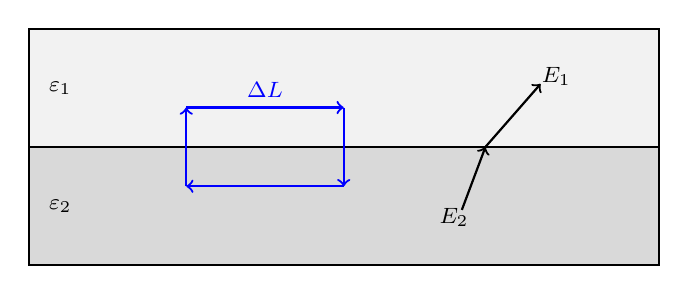
\begin{tikzpicture}
                % Definir colores para las regiones
                \begin{scope}
                    \fill[gray!10] (0,1.5) rectangle (8,3); % Región superior con gris claro
                \end{scope}
                
                \begin{scope}
                    \fill[gray!30] (0,0) rectangle (8,1.5); % Región inferior con gris más oscuro
                \end{scope}
                
                % Dibujar los rectángulos
                \draw [thick] (0,0) rectangle (8,3); % Contorno grande
                \draw [thick] (0,1.5) -- (8,1.5);   % Línea divisoria
        
                % Etiquetas de permitividades
                \node at (0.4,2.25) {\footnotesize $\varepsilon_1$};
                \node at (0.4,0.75) {\footnotesize $\varepsilon_2$};
        
                % Dibujar el camino con flechas en azul
                \draw [thick,->,blue] (2,1) -- (2,2);  % Subida
                \draw [thick,->,blue] (2,2) -- (4,2) node[midway, above] {\footnotesize $\Delta L$}; % Derecha con etiqueta
                \draw [thick,->,blue] (4,2) -- (4,1);  % Bajada
                \draw [thick,->,blue] (4,1) -- (2,1);  % Izquierda
        
                % Flechas negras para representar el campo eléctrico
                \draw [thick,->] (5.5,0.7) -- (5.8,1.5);  % Flecha en el medio 2
                \draw [thick,->] (5.8,1.5) -- (6.5,2.3); % Flecha en el medio 1
        
                % Etiquetas para los campos eléctricos
                \node at (6.7,2.4) {\footnotesize $E_1$};
                \node at (5.4,0.6) {\footnotesize $E_2$};
        
            \end{tikzpicture}
        \end{center}
        
        Se descompone por componente tal que:
        \begin{align}
            E_{1} &= E_{1n} + E_{1t} \\
            E_{2} &= E_{2n} + E_{2t}
        \end{align}
        Utilizando la ecuacion de Faraday integral para el caso electrostatico se tiene:
        \begin{equation}
            \oint \mathbf{E} \cdot d\mathbf{l} = 0
        \end{equation}
        Luego dividiendo por zonas se obtiene:
        \begin{equation}
            E_{1t} \Delta L - E_{1n} \frac{\Delta h}{2}- E_{2n} \frac{\Delta h}{2} - E_{2t} \Delta L + E_{2n} \frac{\Delta h}{2} + E_{1n} \frac{\Delta h}{2} = 0
        \end{equation}
        Notamos que muchos terminos son cancelados dando como resultado que:
        \begin{equation}
            E_{1t} - E_{2t} = 0
        \end{equation}
        Demostrando la primera condición de frontera, por otro lado utilziando la ley de Gauss se tiene que:
        \begin{equation}
            \oint \mathbf{D} \cdot d\mathbf{S} = Q_{f}
        \end{equation}
        Luego expresandola como:
        \begin{equation}
            \oint \mathbf{D} \cdot d\mathbf{S} = \Delta S \cdot \rho_{s}
        \end{equation}
        Tenemos que tomando una superficie como por ejemplo cilindrica:
        \begin{align}
            D_{1n} \Delta S - D_{2n} \Delta S &= \Delta S \cdot \rho_{s}\\
            D_{1n} - D_{2n} &= \rho_{s}
        \end{align}
        Finalmente se obtiene la segunda condición de frontera.Esto se resuelve asumiendo que hay una densidad de carga libre en la superficie de separación de los medios, como por ejemplo la que tendria un condensador, en el caso en que no se tenga una densidad de carga superficial, se logra obtener que:
        \begin{equation}
            D_{1n} = D_{2n}
        \end{equation}
        Similar al caso tangencial.
    \end{enumerate}
    \end{solution}
    %%%%%%%%%%%%%%%%%%%%%%%%%%%
    \question  Para la estructura coaxial de la Figura 1, de longitud \(d\) y diferencia de potencial \(V_{0}\) entre los electrodos en \(r = a\) y \(r = c\), determinar:
    \begin{enumerate}
        \item Potencial \(\phi(r)\) y campo \(E\) en los medios dieléctricos perfectos de permisividad \(\epsilon_{1}\) y \(\epsilon_{2}\).
        \item Carga total \(Q\) en cada uno de los electrodos (demuestre que la magnitud es igual). 
        \item Energía acumulada en campo \(E\) en cada medio dieléctrico.
    \end{enumerate}
    \begin{center}
        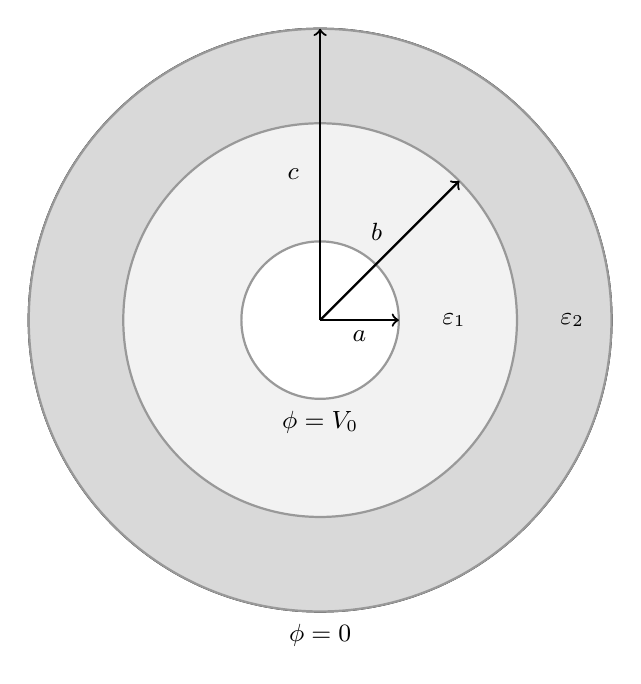
\begin{tikzpicture}
            % Definir los radios
            \def\ra{1}  % Radio interno
            \def\rb{2.5}    % Radio intermedio
            \def\rc{3.7}  % Radio externo
    
            % Dibujar los círculos
            \draw[thick, black] (0,0) circle (\ra);
            \draw[thick] (0,0) circle (\rb);
            \draw[thick] (0,0) circle (\rc);
    
            % Sombreado de la región externa
            \begin{scope}
                \clip (0,0) circle (\rc);
                \fill[gray!30] (-5,-5) rectangle (5,5);
            \end{scope}
        
            \begin{scope}
                \clip (0,0) circle (\rb);
                \fill[gray!10] (-5,-5) rectangle (5,5);
            \end{scope}
            
            \begin{scope}
                \clip (0,0) circle (\ra);
                \fill[white] (-5,-5) rectangle (5,5);
            \end{scope}

            \draw[thick, gray!80] (0,0) circle (\ra);
            \draw[thick, gray!80] (0,0) circle (\rb);
            \draw[thick, gray!80] (0,0) circle (\rc);
            
            % Flechas radiales
            \draw[thick,->] (0,0) -- (\ra,0) node[midway,below] {\small $a$};
            \draw[thick,->] (0,0) -- ({\rb*cos(45)},{\rb*sin(45)}) node[midway,above left,xshift=1pt] {\small $b$};
            \draw[thick,->] (0,0) -- ({\rc*cos(90)},{\rc*sin(90)}) node[midway,left,xshift=-4pt] {\small $c$};

    
            % Etiquetas de materiales
            \node at (\ra+0.7,0) {\small $\varepsilon_1$};
            \node at (\rb+0.7,0) {\small $\varepsilon_2$};
    
            % Condiciones de potencial
            \node at (0,-\ra-0.3) {\small $\phi = V_0$};
            \node at (0,-\rc-0.3) {\small $\phi = 0$};
    
        \end{tikzpicture}
    \end{center}
    %%%%%%%%%%%%%%%%%%%%%%%%%%%
    \begin{solution}
        \begin{enumerate}
            \item Se dice que la geométrica corresponde a una estructura coaxial y por tanto será conveniente el utilizar coordenadas cilindricas.En relacion al enunciado,entre los medios notamos que no existe presencia de carga libre esto implicará que el Laplaciano sea $\sigma_f = 0$.Esto es posible derivarlo de Gauss en presencia de medios (Es importante esta consideracion, dado que la carga ligada esta presente en el desplazamiento y en el parametro $\epsilon$) en su forma  diferencial, es decir:
            \begin{equation}
                \Vec{\nabla} \cdot \textbf{E} = \frac{\rho_f}{\epsilon} 
            \end{equation}
            Se puede interpretar del hecho que cargas puntuales generan zonas de divergencia tanto positivas o negativas alrededor de ellas, pero si no hay cargas en nuestra zona de interés (dentro de la esfera) simplemente podemos asumir por ejemplo que esas cargas son generadas de manera externa y podemos tener un flujo de entrada-salida constante (es decir, una divergencia nula). Luego definimos un potencial para el cual obtenemos su divergencia en coordenadas cilindricas. Dado que el potencial electrico es conservativo ($E = - \nabla \phi$) podemos derivar la ecuacion de Laplace como:
            \begin{equation}
                -\nabla^{2}\phi = \frac{\rho_f}{\epsilon}
            \end{equation}
            Luego tenemos de manera general que el Laplaciano en coordenadas cilíndricas es:
            \begin{equation}
                \nabla^{2}\phi = \frac{1}{\rho} \frac{\partial}{\partial\rho}\left(\rho \frac{\partial\phi}{\partial \rho}\right) + \frac{1}{\rho^{2}}\frac{\partial^{2}\phi}{\partial\theta^{2}} + \frac{\partial^{2}\phi}{\partial z^{2}}
            \end{equation}
            Como se menciono anteriormente,no hay cargas libres no están presente en los medios, por lo tanto podemos hacer la densidad sea nula, por lo que se utiliza la formula del Laplaciano.Debido a que el potencial dependerá de una sola componente (Notar que en $\theta$ la geometria es simetrica al igual que en $z$) es simetrica dada la geometría luego se tendrá que:
            \begin{equation}
                \nabla^{2}\phi(r,\theta, z) =  \nabla^{2}\phi(r)=0
            \end{equation}            
            Luego reemplazando se obtiene mediante integracion directa:
            \begin{equation}
                \frac{1}{\rho} \frac{\partial}{\partial\rho}\left(\rho \frac{\partial \phi}{\partial \rho}\right) = 0
            \end{equation}
            \begin{equation}
                \frac{\partial}{\partial\rho}\left(\rho \frac{\partial \phi}{\partial \rho}\right) = 0
            \end{equation}
            \begin{equation}
                 \left(\rho \frac{\partial \phi}{\partial \rho}\right) = A
            \end{equation}
            \begin{equation}
                 \frac{\partial \phi}{\partial \rho} = \frac{A}{\rho}
            \end{equation}
            \begin{equation}
                 \phi(\rho) = A\int\left(\frac{1}{\rho}\partial\rho\right) + B
            \end{equation}
            \begin{equation}
                  \phi(\rho) = Aln(\rho) + B
            \end{equation}
            Luego se obtiene la expresión para el potencial generalizado, es decir con dos constantes por determinar \textbf{A} y \textbf{B},pero ademas se debe tener en cuenta los dos medios es por esto que el potencial será diferente en estos y por tanto se genera el siguiente par de ecuaciones:
            \begin{equation}
                \phi_{1}(\rho) = Aln(a) + B 
            \end{equation}
            \begin{equation}
                \phi_{2}(\rho) = Cln(c) + D 
            \end{equation}
            Luego podemos utilizar las condiciones de borde para determinar las 4 constantes, comenzamos con los bordes por lo que evaluando:
            \begin{equation}
                \phi_{1}(\rho) = Aln(a) + B = V_{0}
            \end{equation}
            \begin{equation}
                \phi_{2}(\rho) = Cln(c) + D = 0
            \end{equation}
            Dado que el potencial eléctrico \textbf{debe ser continuo},se debe cumplir que $\phi_{1}(\rho=b) =\phi_{2}(\rho=b) $. De esta manera se obtiene otra ecuación:
            \begin{equation}
                \phi_{1}(\rho=b) = \phi_{2}(\rho=b)
            \end{equation}
            \begin{equation}
                Aln(b) + B = ln(b) + D 
            \end{equation}
            Finalmente notamos que tenemos 4 incógnitas, pero solo 3 ecuaciones. Por tanto, debemos obtener alguna más, esto se logra analizando el campo eléctrico:
            \begin{equation}
                E_{1}(\rho) = -\nabla\phi_{1}, \quad E_{2}(\rho) = -\nabla\phi_{2}
            \end{equation}
            Recordando la expresion del gradiente en cilindricas tenemos que:
            \begin{equation}
                \nabla\phi = \frac{\partial \phi}{\partial \rho} \hat{\rho} + \frac{1}{\rho}\frac{\partial \phi}{\partial \theta} \hat{\theta} + \frac{\partial \phi}{\partial z} \hat{z}
            \end{equation}
            Luego reemplazando en la ecuación anterior se obtiene:
            \begin{equation}
                E_{1}(\rho) =-\frac{A}{\rho} \hat{\rho}, \quad E_{2}(\rho) = -\frac{C}{\rho} \hat{\rho}
            \end{equation}
            Luego utilizaremos la condición de borde asociada al desplazamiento eléctrico:
            \begin{equation}
                D_{1n} - D_{2n} = \sigma_{f}
            \end{equation}
            Pero dado que no tenemos carga libre entre los medios luego se tendrá que $\sigma_{f}= 0$ (Esto a diferencia de los electrodos, donde si tenemos presencia de carga libre). Luego reemplazando:
            \begin{equation}
                 D_{1n} = D_{2n}
            \end{equation}
            \begin{equation}
                 \epsilon_{1}V_{1} = \epsilon_{2}V_{2}
            \end{equation}
            \begin{equation}
                 \epsilon_{1}A = \epsilon_{2}C
            \end{equation}
            
            Finalmente se obtienen las 4 ecuaciones que permiten obtener las constantes:
            
            \begin{equation}
            A= \epsilon_{2}\left(\frac{-V_{0} }{\epsilon_{2}ln(\frac{b}{a}) + \epsilon_{1}ln(\frac{c}{b})}\right)
            \end{equation}
            \begin{equation}
            B = V_{0} - Aln(a)
            \end{equation}
            \begin{equation}
            C = \epsilon_{1}\left(\frac{-V_{0}}{\epsilon_{2}ln(\frac{b}{a}) + \epsilon_{1}ln(\frac{c}{b})}\right)
            \end{equation}
            \begin{equation}
            D=-\frac{\epsilon_{1}A}{\epsilon_{2}}\cdot ln(c)
            \end{equation}
        \item Se busca obtener la carga total \textbf{Q} en cada una de las placas de los electrodos, notamos que al ser un condensador ambas placas deberán tener en magnitud la misma carga, pero de signos opuestos. Luego tenemos que aplicando la ley de Gauss:
        \begin{align}
            \oint_{S} \vec{D_{i}} \cdot \vec{ds} &= Q_f\\
        \epsilon_{i} \oint_{S} \vec{E_{i}} \cdot \vec{ds} &= Q_f\\
        \end{align}
        Luego se toma una superficie conveniente tal que envuelva a la carga que buscamos obtener.Por lo tanto considerando un $a \leq r <b$ se tendra:
        \begin{align}
            \oint_{S} \vec{D_{1}} \cdot \vec{ds} &= Q_{a}\\  
            \epsilon_{1} \oint_{S} \frac{A}{\rho} \cdot (\rho) (\partial \theta) (\partial z) &= Q_{a}\\
            \epsilon_{1} A 2 \pi d &= Q_{a}
        \end{align}
        Donde el valor de A es conocido, por lo tanto se obtiene la carga en el electrodo 1.
        \begin{align}
            Q_{a} &= \epsilon_{1}  2 \pi d \cdot \epsilon_{2}\left(\frac{-V_{0} }{\epsilon_{2}ln(\frac{b}{a}) + \epsilon_{1}ln(\frac{c}{b})}\right)\\
        \end{align}
        Si ahora tommos una superficie Gaussiana tal que $ r > c$, se debera cumplir que la carga neta debera ser nula, por lo tanto se tendra que:
        \begin{equation}
            Q_{a} + Q_{c} = 0
        \end{equation}
        Por lo tanto se tendra que:
        \begin{equation}
            Q_{c} = -Q_{a}
        \end{equation}
        Obteniendo lo buscado inicialmente. Tambien puede ser obtenido mediante un radio $b \leq r < c$ como:
        \begin{align}
            \oint_{S} \vec{D_{2}} \cdot \vec{ds} &= Q_{c}\\  
            \epsilon_{2} \oint_{S} \frac{C}{\rho} \cdot (\rho) (\partial \theta) (\partial z) &= Q_{c}\\
            \epsilon_{2} C 2 \pi d &= Q_{c}
        \end{align}
        Luego reemplazando se tendra que, donde anteriormente se demostro que $\epsilon_{1}A = \epsilon_{2}C$ por lo que reemplazando C en lo anterior:
        \begin{align}
            \epsilon_{2} \frac{\epsilon_1}{\epsilon_2}A 2 \pi d &= Q_{c}\\
            \epsilon_{1} A 2 \pi d &= Q_{c}
        \end{align}
        Con lo que se obtiene el valor de la carga en el electrodo 2, siendo la misma expresion. (En este caso el signo aparecera segun como definamos las normales del problema)
        \item Se busca obtener la energía asociada al campo \textbf{E} en cada medio dieléctrico. Teniendo en cuenta la densidad de energia Electrostatica lo cual vendrá dada por la siguiente:
        \begin{equation}
            w_{ei} = \frac{1}{2}\cdot \epsilon_{i} \cdot |E(\rho)|^{2} 
        \end{equation}
        Se observa que esta dependerá de cada medio en el cual estemos evaluando, por tanto haremos la división para cada medio:
        \begin{equation}
            w_{e1} = \frac{1}{2}\frac{\epsilon_{1}A^{2}}{\rho^{2}}
        \end{equation}
        Con lo que integrando sobre todo el volumen se tendrá que la energía total:
        \begin{equation}
            W_{e1} =\int_{v} w_{1}dv
        \end{equation}
        \begin{equation}
            =\int_{0}^{d}  \int_{0}^{2\pi} \int_{a}^{b}\frac{A^{2}}{\rho^{2}} \frac{1}{2}\epsilon_{1} \rho(\partial\rho )(\rho \partial\theta)( \partial z)
        \end{equation}
        \begin{equation}
            = A^{2} \pi d\epsilon_{1} \int_{a}^{b} \frac{1}{\rho} (\partial\rho)
        \end{equation}
        \begin{equation}
            = A^{2}\pi  d \cdot ln\left(\frac{b}{a}\right) \epsilon_{1}
        \end{equation}
        Análogamente para el otro medio se obtendrá que :
        \begin{equation}
            W_{e2}= C^{2} \pi d \cdot ln\left(\frac{c}{b}\right) \cdot \epsilon_{2}
        \end{equation}
    \end{enumerate}
\end{solution}
%%%%%%%%%%%%%%%%%%%%%%%%%%%
\question  Para el dispositivo magnético de la figura 1.4 con dos material de permeabilidad $\mu_{1}$ y $\mu_{2}$, con espesores $d_{1}$ y $d_{2}$ y sección transversal circular de radio a, determinar: 
\begin{enumerate} 
    \item Potencial magnético escalar $\phi_{m}(z)$ en los medios 1 y 2,y campos $H_{1}$ y $H_{2}$ 
    \item Inductancia L del enrollado
    \item Energía magnética acumulada $W_{m}$ en los medios 1 y 2 
\end{enumerate}
\begin{center}
    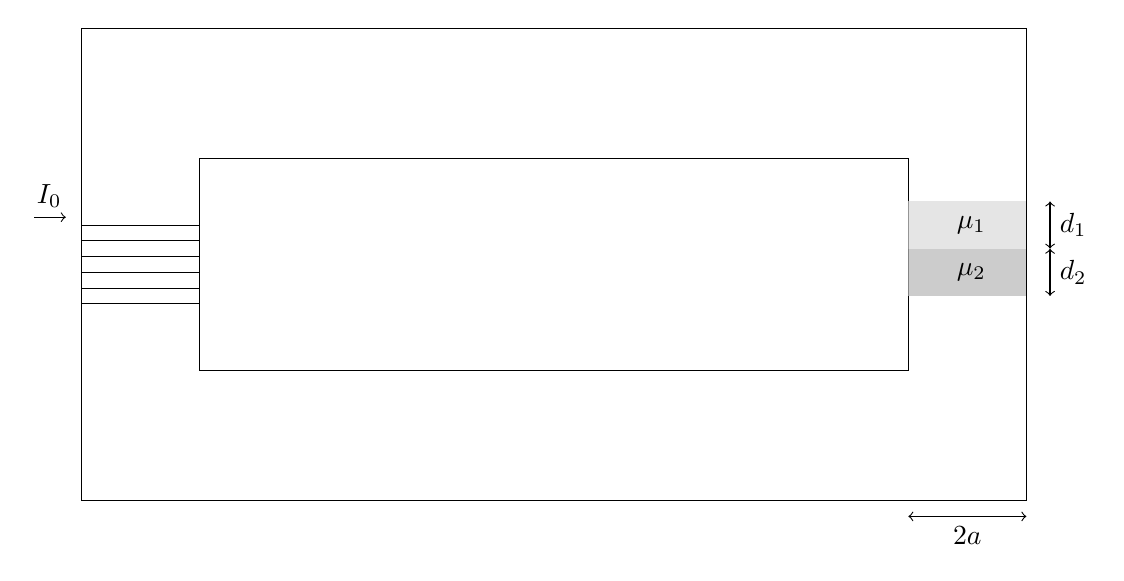
\begin{tikzpicture}
        % Dimensiones
        \def\a{1} % Aumentando la longitud horizontal
        \def\dOne{0.6}
        \def\dTwo{0.6}
        \def\coreWidth{6} % Reduciendo el ancho del núcleo ferromagnético
        \def\coreHeight{3}
        \def\gap{0.15} % Reduciendo el ancho del gap
        \def\offsetY{-0.4} % Ajuste para mover d1 y d2 más abajo
        \def\innerCoreWidth{9} % Haciendo el núcleo interno más ancho
    
        % Dibujar el núcleo
        \draw (-\coreWidth, -\coreHeight) rectangle (\coreWidth, \coreHeight);
        \draw (-\innerCoreWidth/2, -\coreHeight/2 + \gap) rectangle (\innerCoreWidth/2, \coreHeight/2 - \gap);
        
        % Dibujar la sección sombreada de d1
        \begin{scope}
            \clip (\innerCoreWidth/2, \offsetY+\dTwo) rectangle (\coreWidth, \offsetY+\dOne+\dTwo);
            \fill[gray!20] (\innerCoreWidth/2, \offsetY+\dTwo) rectangle (\coreWidth, \offsetY+\dOne+\dTwo);
        \end{scope}
        
        % Dibujar la sección sombreada de d2
        \begin{scope}
            \clip (\innerCoreWidth/2, \offsetY) rectangle (\coreWidth, \offsetY+\dTwo);
            \fill[gray!40] (\innerCoreWidth/2, \offsetY) rectangle (\coreWidth, \offsetY+\dTwo);
        \end{scope}
        
        % Etiquetas
        \draw[<->] (\coreWidth+0.3, \offsetY) -- ++(0, \dTwo) node[midway,right] {$d_2$};
        \draw[<->] (\coreWidth+0.3, \offsetY+\dTwo) -- ++(0, \dOne) node[midway,right] {$d_1$};
        \draw[<->] (\innerCoreWidth/2, -\coreHeight-0.2) -- ++(\a+0.5, 0) node[midway,below] {$2a$};
        
        % Bobina (líneas horizontales)
        \foreach \y in {-0.5,-0.3,-0.1,0.1,0.3,0.5} {
            \draw (-\coreWidth,\y) -- (-\innerCoreWidth/2,\y);
        }

        % Corriente
      \draw[->] (-\coreWidth-0.6, 0.6) -- (-\coreWidth-0.2, 0.6) node[above, xshift=-6pt] {$I_0$};

       % Etiquetas de permeabilidad
        \node at (\coreWidth-0.7, \offsetY+\dTwo+\dOne/2) {$\mu_1$}; % En la zona d1
        \node at (\coreWidth-0.7, \offsetY+\dTwo/2) {$\mu_2$}; % En la zona d2
    \end{tikzpicture}
\end{center}
%%%%%%%%%%%%%%%%%%%%%%%%%%%
\begin{solution}
    \begin{enumerate}
        \item Se busca obtener el potencial magnético escalar $\phi_{m}$, el cual es posible definirlo en condiciones de \textbf{flujo magnético nulo} principalmente y en otro tipo de condiciones. Este potencial se deberá obtener para los medios 1 y 2.

        \textit{Observación: No confundir con el potencial escalar eléctrico $\phi_{e}$})
    
        Se observa la presencia de un núcleo ferromagnético (Muy usados en motores) que implicará una permeabilidad magnética casi infinita ($\mu \rightarrow \infty$). Además, en el núcleo ferromagnético tenemos lo siguiente con relación con respecto a la intensidad magnética: 
        \begin{align}
            H = \frac{1}{\mu} B 
        \end{align}
        Dada la consideración anterior se tendrá que $H \rightarrow 0 $, es de importancia considerar que esta relación la podemos realizar dado que no estamos en presencia de un desplazamiento eléctrico variable en el tiempo $\textbf{D}$ (ver ecuaciones de Maxwell). Debido a lo anterior, no se tendrá una corriente superficial en el núcleo: 
        \begin{align}
            \nabla \times H = J  
        \end{align}
        Siendo de esta manera consistente, se tendrá: 
        \begin{align}
            \nabla \times H = 0  
        \end{align}
        De esta manera similar al campo vectorial eléctrico se podrá definir un potencial escalar para la intensidad de campo magnético $H$ tal que:
        \begin{equation}
            H = -\nabla \phi_{m} 
        \end{equation}
        En base a esto podemos verificar de manera directa que cumple con la ecuación de Laplace:\\
        \begin{align}
            \nabla \cdot B = \nabla \cdot \mu H= 0 
        \end{align}
        Lo cual es equivalente a 
        \begin{align}
            \nabla \cdot H &= 0\\
            \nabla \cdot (-\nabla \phi_{m}) &= 0\\
            \nabla^{2} \phi_{m}= 0 
        \end{align}
        Con lo que finalmente se logra definir un potencial magnético. Luego podemos analizar el tipo de coordenadas a utilizar, se observa que es de conveniencia el utilizar coordenadas cilíndricas, con lo que:
        \begin{align}
            \nabla^{2}\phi_{m} = \frac{1}{\rho} \frac{d}{d\rho}\left(\rho \frac{d\phi}{d\rho}\right) + \frac{1}{\rho^{2}}\frac{d^{2}\phi}{d\rho^{2}} + \frac{d^{2}\rho}{dz^{2}}
        \end{align}
        Se tendrá que el potencial escalar magnético dependerá de una sola dirección, es decir, $\phi_{m}(z)$ por tanto:
        \begin{align}
            \nabla^{2} \phi(z) = \frac{d^{2} \phi_{m}}{dz^{2}} &= 0\\
            \frac{d^{2} \phi_{m}}{dz^{2}} &= 0\\
            \frac{d\phi_{m}}{dz} &= A\\
            \phi_{m}(z) &= Az + B
        \end{align}
        Se obtiene la forma del campo magnético escalar. Luego tenemos la presencia de dos medios, por lo tanto deberemos hacer la distinción entre cada uno de estos.
        \begin{align}
            \phi_{m1}(z) &= Az + B \\
            \phi_{m2}(z) &= Cz + D 
        \end{align}
        Con lo que de manera análoga se deberá encontrar 4 ecuaciones tal que permitan despejar estas constantes. Usando las condiciones de borde entregadas.
        \subsubsection*{\underline{Medio 1}}
        \begin{align}
            \phi_{m1}(z=(d_{1} + d_{2}))  &= A(d_{1} + d_{2}) + B \\&= N I_{0} 
        \end{align}
        \subsubsection*{\underline{Medio 2}}
        \begin{align}
            \phi_{m2}(z=0)  &= C\cdot 0+ D \\&= 0
        \end{align}
        Lo que implicará de manera directa que $D=0$. Se tendrá además que el campo magnético escalar deberá ser continuo.
        \begin{align}
            \phi_{m1}(z=d_{2}) &=\phi_{m2}(z=d_{2}) \\ A d_{2} + B &= C d_{2} 
        \end{align}
        Dado que se busca el obtener otra ecuación, Se utiliza el gradiente en cilindricas, el cual de manera general se define como:
        \begin{align}
            \nabla \phi = \frac{\partial \phi}{\partial \rho} \hat{\rho} + \frac{1}{\rho}\frac{\partial \phi}{\partial \theta} \hat{\theta} + \frac{\partial \phi}{\partial z} \hat{z}
        \end{align}
        Luego reemplazando en la ecuación anterior se obtiene:
        \begin{align}
            H_{1} &= - \nabla \phi_{m1} &  
            H_{2} &= - \nabla \phi_{m2}\\
             H_{1}&= -\frac{d\phi_{m1}}{dz} &   H_{2}&= -\frac{d\phi_{m2}}{dz}\\
             &= -A  &  &= -C
        \end{align}
        De esta manera tenemos que por condición de borde y dado que el campo tiene solo componente normal en la zona de interés se cumple:
        \begin{align}
            B_{1n} &= B_{2n}\\
            \mu_{1}H_{1} &=  \mu_{2}H_{2}\\
            \mu_{1}A &=  \mu_{2}C   
        \end{align}
        Luego se puede plantear 4 set de ecuaciones las cuales vendrán dados:
        \begin{align}
            NI_{0} &= A(d_{1} + d_{2}) + B\\
            D&=0\\
            \mu_{1}A &=  \mu_{2}C\\
            Ad_{2} + B &= Cd_{2}
        \end{align}
        Luego despejando las variables se obtiene lo siguiente:
        \begin{align}
        A &= \frac{\mu_{2} N I_{0}}{d_{2}(\mu_{1} + \mu_{2})}\\
         B&= \left(\frac{NI_{0}\mu_{1}}{d_{2}(\mu_{1} + \mu_{2})}\right) d_{2} - \left(\frac{\mu_{2} N I_{0}}{d_{2}(\mu_{1} + \mu_{2})}\right)d_{1}\\
         C&= \frac{NI_{0}\mu_{1}}{d_{2}(\mu_{1} + \mu_{2})}\\
         D&=0
        \end{align}
        Finalmente se despejan que permiten el determinar tanto $H_{1} , H_{2},\phi_{m1}$  y $\phi_{m2} $.
        \item Se busca obtener la inductancia L que vendrá caracterizada por la siguiente expresión: 
        \begin{align}
            L = \frac{\phi N}{I}
        \end{align}
        Donde $\phi$ corresponde al flujo magnético y nos da una idea de cuando campo magnético hay en una superficie dada y deberá por tanto, considerar ambos medios:
        \begin{align}
            \phi_{1} &= \int B_{1} dS\\
                     &= \mu_{1} \int_{S} H_{1} dS\\
                     &= \mu_{1} \int_{0}^{2\pi} \int_{0}^{a} A (-\hat{z}) \cdot r (dr) (d\theta) (-\hat{z})  \\
                     &= \mu_{1}  \pi a^{2} A\\
                     &= \mu_{1}\pi a^{2} \left(\frac{\mu_{2} N I_{0}}{d_{2}(\mu_{1} + \mu_{2})}\right)
          \end{align}
        De manera análoga tenemos que el flujo para la otra superficie vendrá dado por:
        \begin{align}
            \phi_{2} &= \int B_{2} dS\\
                     &= \mu_{2} \int_{S} H_{2} dS\\
                     &= \mu_{2} \int_{0}^{2\pi} \int_{0}^{a} C (-\hat{z}) \cdot r (dr) (d\theta) (-\hat{z})  \\
                     &= \mu_{2}  \pi a^{2} C\\
                     &= \mu_{2}\pi a^{2} \left(\frac{\mu_{1} N I_{0}}{d_{2}(\mu_{1} + \mu_{2})}\right)
          \end{align}
        Una vez obtenido el flujo magnético para ambos medios se logra obtener la inductancia utilizando la expresión:
        \begin{align}
            L = \frac{\phi N}{I_{0}}
        \end{align}
        \textit{Observación: Es importante considerar que es posible tomar cualquier flujo para calcular la inductancia, esto debido a que por condiciones de borde se tendrá que $B_{1} = B_{2}$ y por tanto el utilizar una u otra es análogo.}
        \item Debemos obtener la energía magnética acumulada $W_{m}$ en ambos medios, para esto se utilizará la siguiente expresión:
        \begin{equation}
            w_{m} = \frac{1}{2} \mu H^{2}
        \end{equation}
        Luego como se quiere la energía magnética se integra sobre un volumen tal que:
        \subsubsection*{\underline{Medio 1}}
        \begin{align}
            W_{m1} &= \frac{\mu_{1}}{2}\int_{v} H_{1}^{2} dv\\
                   &= \frac{\mu_{1}}{2}A^{2} \int_{d2}^{d1+d2} \int_{0}^{2\pi} \int_{0}^{a} r (dr) (d\theta) (dz)\\
                   &=\frac{\mu_{1}}{2} A^{2} \pi a^{2}d_{2} 
        \end{align}
        \subsubsection*{\underline{Medio 2}}
        \begin{align}
            W_{mw} &= \frac{\mu_{w}}{2}\int_{v} H_{2}^{2} dv\\
                   &= \frac{\mu_{2}}{2}C^{2} \int_{0}^{d1} \int_{0}^{2\pi} \int_{0}^{a} r (dr) (d\theta) (dz)\\
                   &=\frac{\mu_{2}}{2} C^{2} \pi a^{2}d_{1} 
        \end{align}
        Finalmente se obtienen las energías acumuladas en los dos diferentes medios dado que A y C son términos conocidos.
    \end{enumerate}
\end{solution}
\end{questions}
\newpage
%%%%%%%%%%%%%%%%%%%%%%%%%%%

\end{document}